\begin{abstract}

GLM-OCR is an efficient 0.9B-parameter compact multimodal model designed for real-world document understanding. It combines a 0.4B-parameter CogViT visual encoder with a 0.5B-parameter GLM language decoder, achieving a strong balance between computational efficiency and recognition performance. To address the inefficiency of standard autoregressive decoding in deterministic OCR tasks, GLM-OCR introduces a Multi-Token Prediction (MTP) mechanism that predicts multiple tokens per step, significantly improving decoding throughput while keeping memory overhead low through shared parameters. At the system level, a two-stage pipeline is adopted: PP-DocLayout-V3 first performs layout analysis, followed by parallel region-level recognition. Extensive evaluations on public benchmarks and industrial scenarios show that GLM-OCR achieves competitive or state-of-the-art performance in document parsing, text and formula transcription, table structure recovery, and key information extraction. Its compact architecture and structured generation make it suitable for both resource-constrained edge deployment and large-scale production systems.

\end{abstract}

\begin{figure}[!h]
\centering
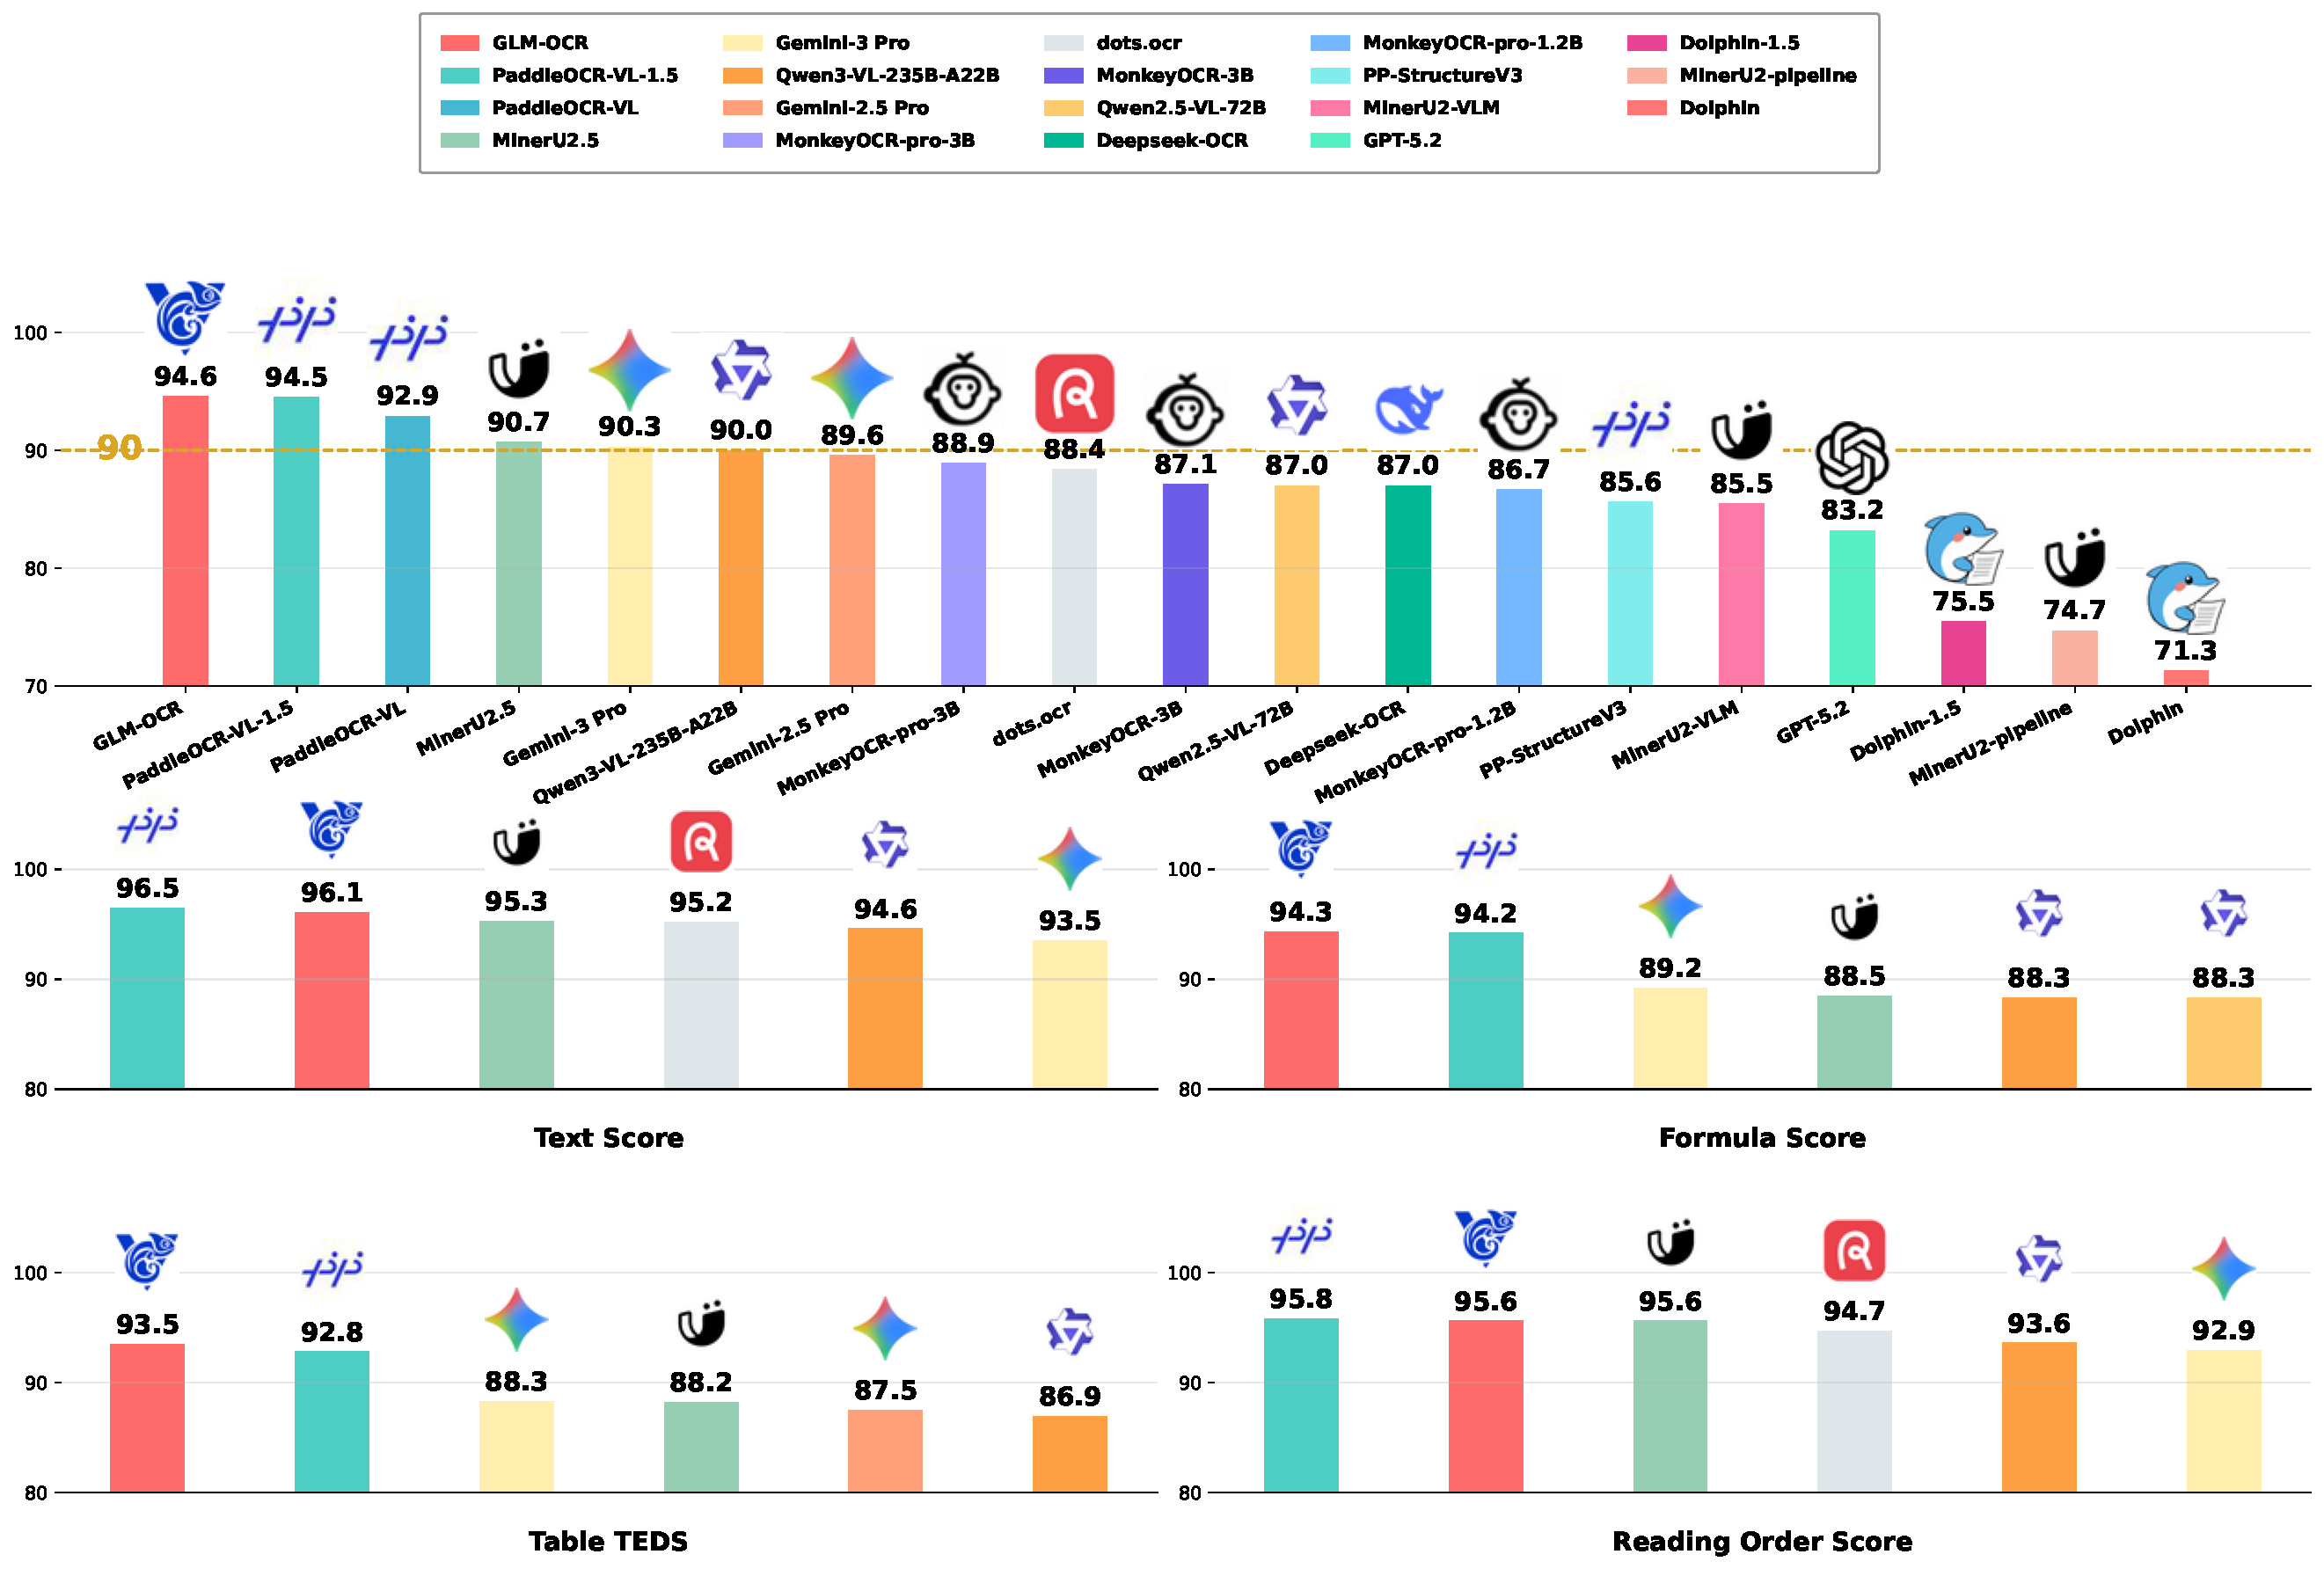
\includegraphics[width=\linewidth]{assets/omnidocbench_vis.pdf}
\caption{Performance of GLM-OCR on OmniDocBench v1.5.}
\label{fig:eval_comparison}
\end{figure}